\documentclass[]{scrartcl}
%\usepackage{ucs}

\usepackage[utf8]{inputenc}
\usepackage[T1]{fontenc}
\usepackage{ngerman}
\usepackage{subcaption}
\usepackage[automark]{scrpage2}
\usepackage{listings}
\usepackage{tabularx}
\usepackage{graphicx}
\usepackage{hyperref}

\usepackage[usenames,dvipsnames]{xcolor}

\pagestyle{scrheadings}


%opening
\title{SPV Projekt}

\author{Timo Briddigkeit \and Johannes Selymes}
\date{\today{}, Hagenberg}

\ifoot{Briddigkeit, Selymes}
\cfoot[]{SPV SS15}
\ofoot{\pagemark}

\begin{document}

\maketitle
\newpage
\tableofcontents
\newpage


\definecolor{bluekeywords}{rgb}{0,0,1}
\definecolor{greencomments}{rgb}{0,0.5,0}
\definecolor{redstrings}{rgb}{0.64,0.08,0.08}
\definecolor{xmlcomments}{rgb}{0.5,0.5,0.5}
\definecolor{types}{rgb}{0.17,0.57,0.68}

\lstset{language=[Sharp]C,
captionpos=b,
numbers=left, %Nummerierung
numberstyle=\tiny, % kleine Zeilennummern
frame=lines, % Oberhalb und unterhalb des Listings ist eine Linie
showspaces=false,
showtabs=false,
breaklines=true,
showstringspaces=false,
breakatwhitespace=true,
escapeinside={(*@}{@*)},
commentstyle=\color{greencomments},
morekeywords={partial, var, value, get, set},
keywordstyle=\color{bluekeywords},
stringstyle=\color{redstrings},
basicstyle=\ttfamily\small,
tabsize=2,
inputencoding={ansinew}
}

\section{Einleitung}
Grundlage für die heute gänigen Quadrocopter sind Fortschritte in der Elektronik und Sensorik, die auf dem Markt ab etwa 2000 verfügbar waren und ab 2004 in Serienmodellen erschienen: Leistungsfähige Mikrocontroller werten die Daten von Gyroskopen aus und können so Kippmomente – die höher und plötzlicher auftreten als bei Hubschraubern, da der Auftriebsschwerpunkt meist in der Rotorebene liegt – automatisch ausregeln.\\
\\
Dabei kommen Gyroskopsensoren auf Piezo-Basis oder MEMS (microelectromechanical systems) zur Messung der Winkelgeschwindigkeit zum Einsatz, die von dem Prozessor benutzt werden, um durch Drehzahlregelung der Elektromotoren die Drehraten zu dämpfen, womit das Fluggerät steuerbar bleibt.\\
\\
In diesem Projekt wird es ermöglicht, die Parameter der Regelung des Quadrocopters vom Computer aus einzustellen. Es wird dazu ein Server am Quadrocopter eingerichtet und eine WPF-Gui für das Windowssystem am Computer erstellt.

\newpage

\section{QuadServer}
Auf dem Quadrocopter ist ein BeagleBone, auf welchem ein gentoo Linux läuft, installiert. Auf diesem Linux wird eine Applikation erstellt, welche als Server für das QuadcopterGui verwendet wird. Um die Applikation später in der Regelung einbinden zu können, wird der Server in einen Thread verpackt, der zyklisch Daten vom Socket abruft. Wenn Daten erhalten werden, werden diese geparst und die Parameter werden in das globale Parameter Singleton geschrieben. Dann wird noch ein Flag gesetzt, dass die Parameter geändert wurden, was dann später in der Regelung abgefragt wird. 


\section{QuadcopterGui}
QuadcopterGui ist ein Prototyp für eine WPF-Anwendung, in der ein PID-Regler (\textbf{P}roportional, \textbf{I}ntegral, \textbf{D}ifferential) mit Winkel und Winkelgeschwindigkeit angesteuert werden kann. Die Anwendung baut eine Verbindung zum QuadServer auf und schickt durch Betätigung des Send-Buttons PID-Regelwerte an den Quadserver, welche sich über sog. Slider einstellen lassen. Eine Textbox links und rechts vom Slider definiert den Minimal- bzw. Maximalwert des entsprechenden Regelwertes.\\
Die Übergabe der Minimal- bzw. Maximalwerte erfolgt über sog. Databinding an den Slider.

\begin{figure}[h]
\includegraphics[scale=1]{img/gui.png} 
\caption{Screenshot der QuadcopterGui Anwendung}
\end{figure}

\newpage
\section{Netzwerkkommunikation}
Die beiden Anwendungen kommunizieren über eine TCP/IP Verbindung. Dabei versendet die QuadcopterGui ihre Daten in einem JSON-Format, ein kompaktes Datenformat in einer einfach lesbaren Textform zum Zweck des Datenaustauschs zwischen Anwendungen, welche vom QuadServer geparst werden. Das JSON-Format ist notwendig, um das Endian-Problem zu umgehen, welches sich zwischen unterschiedlichen Computersystem stellen kann. Während heutige PC-Systeme in der Regel Little-Endian sind, sind ARM-Prozessoren, welche häufig im Embedded-Bereich anzutreffen sind, Bi-Endian Systeme. Die eigentliche TCP/IP Kommunikation erfolgt wie nachfolgend dargestellt drahtlos.
\begin{figure}[h]
\centering
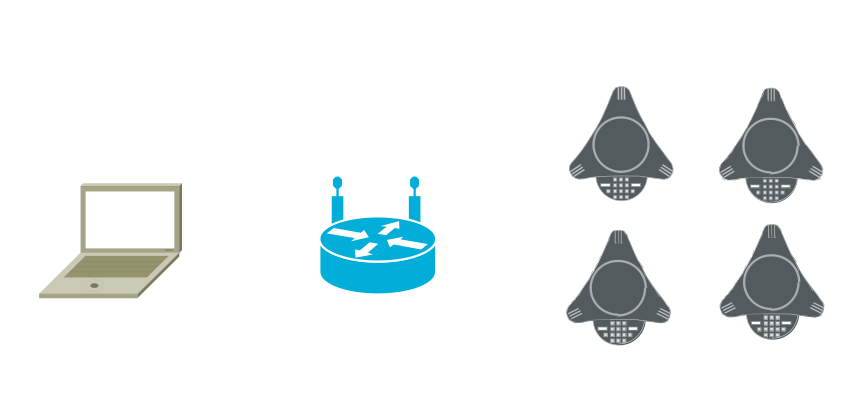
\includegraphics[scale=0.5]{img/comm.png} 
\caption{Netzwerkkommunikation}
\end{figure}

\newpage
\section{Testausgaben}
Hier sieht man auf der linken Seite das GUI und auf der rechten Seite das Linux des BeagleBones mit SSH verbunden. Wie zu sehen ist, fehlt noch der N Parameter, welcher aber dank JSON noch leicht hinzugefügt werden kann.
\begin{figure}[ht]
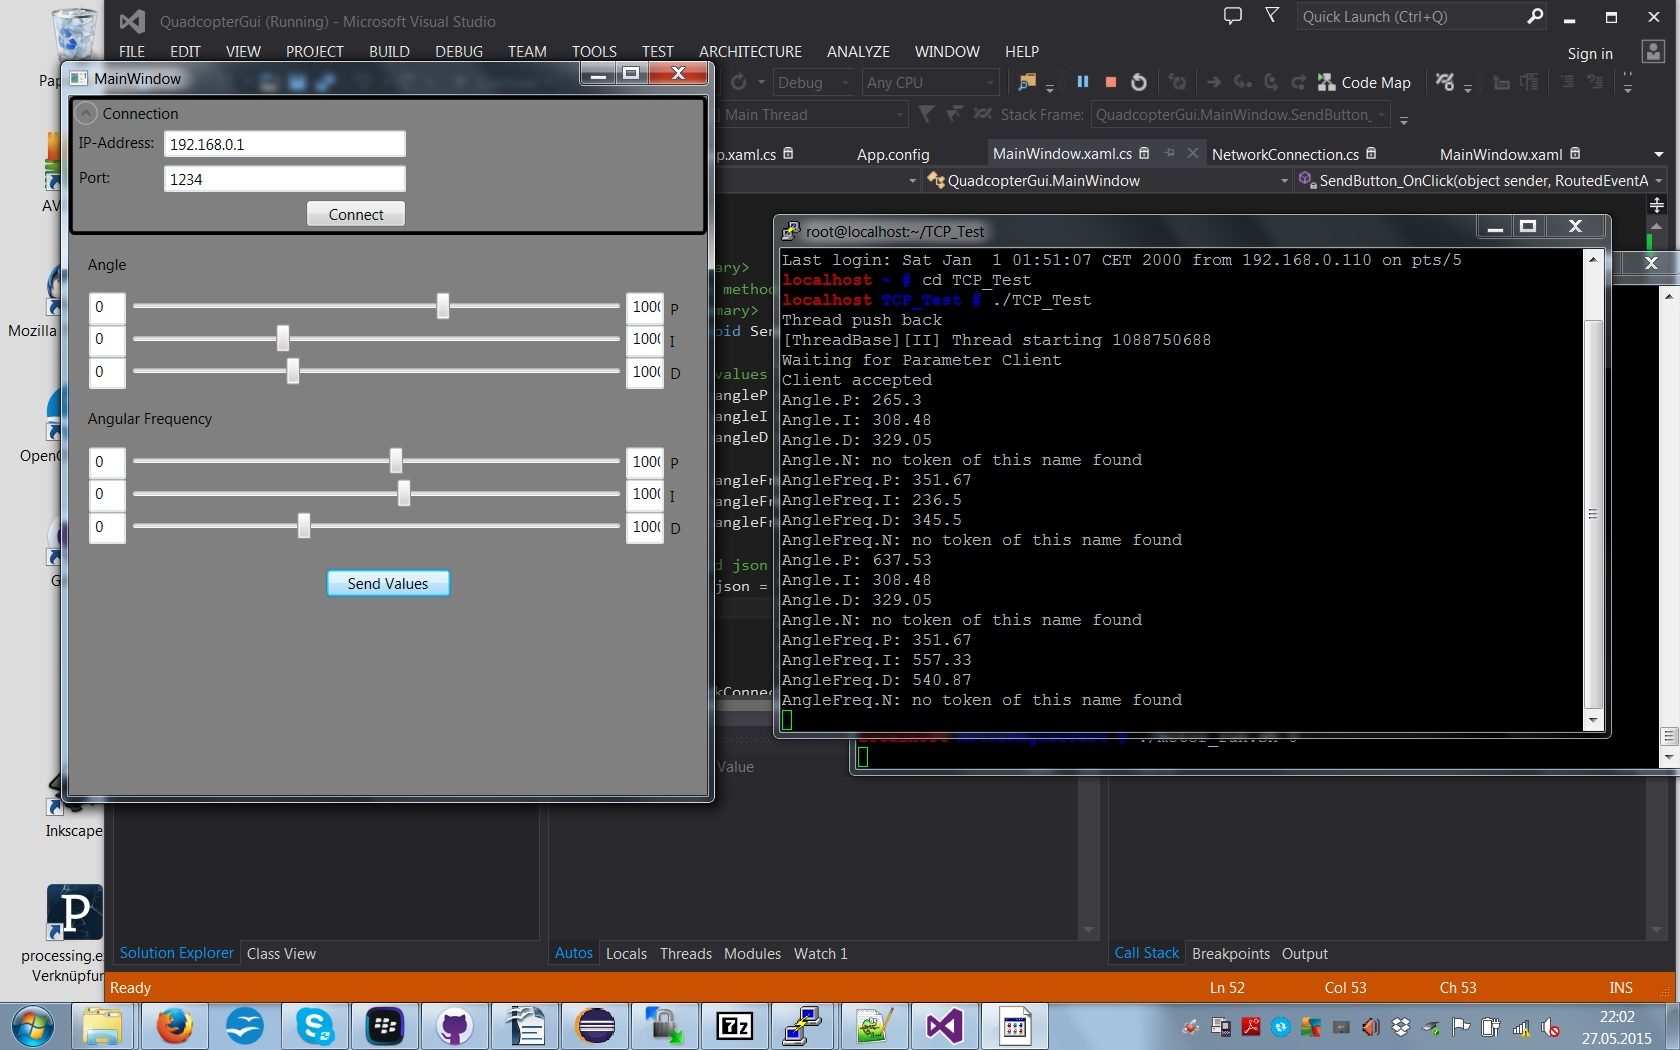
\includegraphics[scale=0.4]{img/screen.jpg} 
\caption{Screenshot der Anwendung}
\end{figure}

\newpage
\section{Code des Servers}
Einige Dateien werden der Übersichtlichkeit halber nicht ins PDF mitaufgenommen.
\lstinputlisting[language=C++]{../../../QuadServer/TCP_Test/src/JSONParser.h}
%\lstinputlisting[language=C++]{../../../QuadServer/TCP_Test/src/JSONParser.c}
\lstinputlisting[language=C++]{../../../QuadServer/TCP_Test/src/Parameters.h}
\lstinputlisting[language=C++]{../../../QuadServer/TCP_Test/src/Parameters.cpp}
\lstinputlisting[language=C++]{../../../QuadServer/TCP_Test/src/SocketCommunication.h}
%\lstinputlisting[language=C++]{../../../QuadServer/TCP_Test/src/SocketCommunication.cpp}
\lstinputlisting[language=C++]{../../../QuadServer/TCP_Test/src/ThreadBase.h}
\lstinputlisting[language=C++]{../../../QuadServer/TCP_Test/src/ThreadBase.cpp}
\lstinputlisting[language=C++]{../../../QuadServer/TCP_Test/src/ParameterUpdateThread.h}
\lstinputlisting[language=C++]{../../../QuadServer/TCP_Test/src/ParameterUpdateThread.cpp}
\lstinputlisting[language=C++]{../../../QuadServer/TCP_Test/src/TCP_TestConnection.h}
\lstinputlisting[language=C++]{../../../QuadServer/TCP_Test/src/TCP_TestConnection.cpp}

\section{Code der GUI}
\lstinputlisting{../../../QuadcopterGui/QuadcopterGui/NetworkConnection.cs}
\lstinputlisting{../../../QuadcopterGui/QuadcopterGui/MainWindow.xaml.cs}
\lstinputlisting[language=xml]{../../../QuadcopterGui/QuadcopterGui/MainWindow.xaml}

\listoffigures
%\lstlistoflistings

\end{document}